\newpage
\setcounter{dang}{0}

\section{BA ĐƯỜNG CONIC}
\Opensolutionfile{ans}[ans/ans-conic]
\subsection{Elip}
\begin{dang}{Elip}
	Từ phương trình chính tắc của elip $(E)$ tìm $a$, $b$, $c$; từ đó suy ra các yếu tố của elip $(E)$ và ngược lại.
\subsubsection{Khái niệm elip}
\immini{Cho hai điểm cố định $ F_1 $, $ F_2 $ và một độ dài không đổi $ 2a $ lớn hơn $ F_1F_2 $. Elip $ (E) $ là tập hợp các điểm $ M $ trong mặt phẳng sao cho $$F_1M+F_2M=2a.$$
	Các điểm $ F_1 $ và $ F_2 $ gọi là các tiêu điểm của elip.\\
	Độ dài $ F_1F_2 = 2c $ gọi là tiêu cự của elip ($ a>c $).
}
{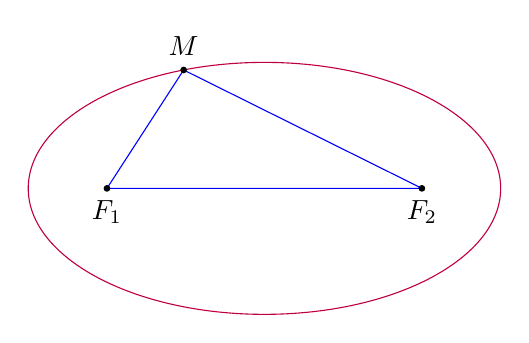
\begin{tikzpicture}[line join = round, line cap = round,>=stealth,scale=1]
		%Phạm Đức Thiệu - Hình số - Trang số.
		\draw[color=purple](0,0)coordinate(O)ellipse(3 and 1.6);
		\draw[color=blue](-2,0)coordinate(F_{1})--(110:3 and 1.6)coordinate(M)--(2,0)coordinate(F_{2}) (F_{1})--(F_{2});
		\foreach \p/\g in {M/90,F_{1}/-90,F_{2}/-90}
		\draw[fill=black](\p)circle (1pt)node [shift={(\g:.3)}] {$\p$};
	\end{tikzpicture}
}
\noindent
\subsubsection{Phương trình chính tắc của elip}
\immini{Cho elip $ (E) $ có các tiêu điểm $ F_1 $ và $ F_2 $ và đặt $ F_1F_2 = 2c $. Chọn hệ trục tọa độ Oxy sao cho $ F_1(-c; 0) $ và $ F_2(c; 0) $.
	$$M(x;y) \in (E) \Leftrightarrow \dfrac{x^2}{a^2}+\dfrac{y^2}{b^2}=1\;(1)$$ trong đó $b=\sqrt{a^2-c^2}$.\\
	Phương trình (1) gọi là phương trình chính tắc của elip.
}
{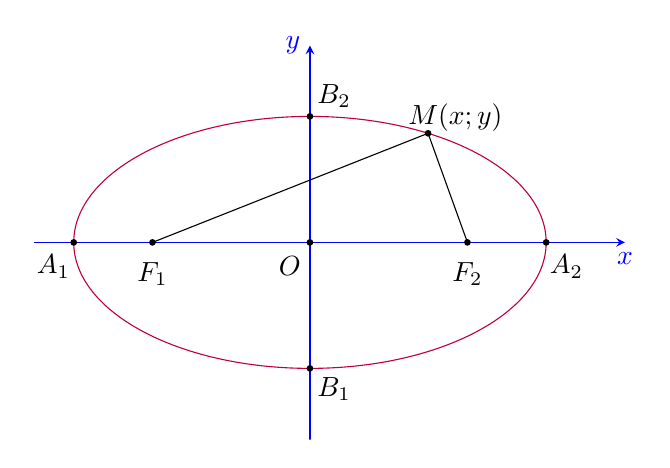
\begin{tikzpicture}[line join = round, line cap = round,>=stealth,scale=1]
		%Phạm Đức Thiệu - Hình số - Trang số.
		\draw[color=blue,-stealth](-3.5,0)--(4,0)node[below]{$x$};
		\draw[color=blue,-stealth](0,-2.5)--(0,2.5)node[left]{$y$};
		\draw[color=purple](0,0)coordinate(O)ellipse(3 and 1.6);
		\draw (-3,0)coordinate(A_1);
		\draw (3,0)coordinate(A_2);
		\draw (0,-1.6)coordinate(B_1);
		\draw (0,1.6)coordinate(B_2);
		\draw (-2,0)coordinate(F_{1})--(60:3 and 1.6)coordinate(M{(x;y)})--(2,0)coordinate(F_{2});
		\foreach \p/\g in {M{(x;y)}/30,F_{1}/-90,F_{2}/-90,O/-130,A_1/-130,A_2/-50,B_1/-40,B_2/40}
		\draw[fill=black](\p)circle (1pt)node [shift={(\g:.4)}] {$\p$};
	\end{tikzpicture}
}
\begin{note}
	\immini{
		\begin{itemize}[$ \bullet $]
			\item Elip $ (E) $ cắt $ Ox $ tại hai điểm$  A_1(-a; 0) $, $ A_2(a; 0) $ và cắt $ Oy $ tại hai điểm $ B_1(0; -b) $, $ B_2(0; b) $.
			\item Các điểm $ A_1 $, $ A_2 $, $ B_1 $, $ B_2 $ gọi là các đỉnh của elip.
			\item Đoạn thẳng $ A_1A_2 = 2a $ gọi là trục lớn, đoạn thẳng $ B_1B_2 = 2b $ gọi là trục nhỏ của elip.
			\item Giao điểm $ O $ của hai trục là tâm đối xứng của elip.
			\item Nếu $M(x; y) \in (E)$ thì $|x| \leq a$, $|y| \geq b$.
		\end{itemize}
	}
	{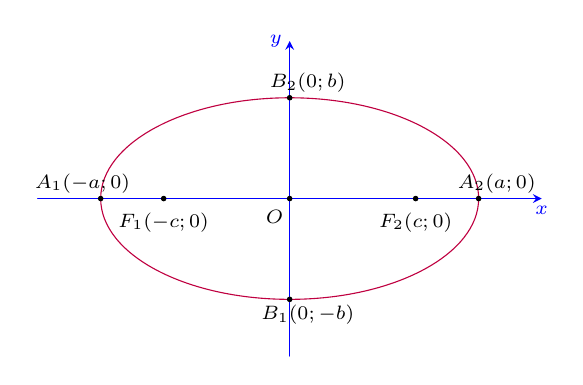
\begin{tikzpicture}[line join = round, line cap = round,>=stealth,scale=0.8]
			%Phạm Đức Thiệu - Hình số - Trang số.
			{\scriptsize \draw[color=blue,-stealth](-4,0)--(4,0)node[below]{$x$};
				\draw[color=blue,-stealth](0,-2.5)--(0,2.5)node[left]{$y$};
				\draw[color=purple](0,0)coordinate(O)ellipse(3 and 1.6);
				\draw (-3,0)coordinate(A_1{(-a;0)});
				\draw (3,0)coordinate(A_2{(a;0)});
				\draw (0,-1.6)coordinate(B_1{(0;-b)});
				\draw (0,1.6)coordinate(B_2{(0;b)});
				\draw (-2,0)coordinate(F_{1}{(-c;0)});
				\draw (2,0)coordinate(F_{2}{(c;0)});
				\foreach \p/\g in {F_{1}{(-c;0)}/-90,F_{2}{(c;0)}/-90,O/-130,A_1{(-a;0)}/140,A_2{(a;0)}/40,B_1{(0;-b)}/-40,B_2{(0;b)}/40}
				\draw[fill=black](\p)circle (1pt)node [shift={(\g:.3)}] {$\p$};}
		\end{tikzpicture}
	}
\end{note}

\end{dang}
\subsubsection{Ví dụ mẫu}
\begin{vd}%[Phạm Đức Thiệu, dự án CĐ_Toán10]%[0H3B3-1]
	\begin{enumerate}
		\item [a)] Cho elip $ (E) $: $\dfrac{x^2}{25}+\dfrac{y^2}{9}=1$. Tìm tâm sai của $ (E) $.
		\item [b)] Một elip có độ dài trục lớn bằng $ 26 $, tâm sai $e=\dfrac{12}{13}$. Tìm độ dài trục nhỏ của elip $ (E) $.
	\end{enumerate}
	\loigiai{
		\begin{itemize}
			\item [a)] Trong phương trình chính tắc của elip $ (E) $, ta có:
			$$a^2=25;\ b^2=9 \Rightarrow c^2=a^2-b^2=25-9=16\Rightarrow c=\sqrt{16}=4.$$
			Do đó, tâm sai của elip $ (E) $ là: $ e=\dfrac{c}{a}=\dfrac{4}{5} $.
			\item [b)]
			Độ dài trục lớn $2a=26\Rightarrow a=13$.\\
			Tâm sai $e=\dfrac{c}{a}=\dfrac{12}{13}\Rightarrow c=a.e=13\cdot\dfrac{12}{13}=12$.\\
			Suy ra $b^2=a^2-c^2=13^2-12^2=169-144=25\Rightarrow b=\sqrt{25}=5$.\\
			Vậy độ dài trục bé của elip $ (E) $ là: $ 2b=2.5=10 $.
		\end{itemize}
	}
\end{vd}
\begin{note}
	Tâm sai $e=\dfrac{c}{a}$.
\end{note}

\begin{vd}%[Phạm Đức Thiệu, dự án CĐ_Toán10]%[0H3B3-1]%[0H3B3-2]
	Cho elip $ (E) $ có độ dài trục lớn bằng $ 10 $, tỉ số giữa tiêu cự và độ dài trục lớn là $\dfrac{2}{5}$.
	\begin{itemize}
		\item [a)] Tính độ dài trục nhỏ của elip $ (E) $.
		\item [b)] Viết phương trình chính tắc của elip $ (E) $.
	\end{itemize}
	\loigiai{
		Độ dài trục lớn $2a=10\Rightarrow a=5$.\\
		Tỉ số giữa tiêu cự và độ dài trục lớn là $\dfrac{2c}{2a}=\dfrac{c}{a}=\dfrac{2}{5}\Rightarrow c=a\cdot e=5\cdot\dfrac{2}{5}=2$.\\
		\begin{itemize}
			\item [a)]
			Ta có: $b^2=a^2-c^2=5^2-2^2=25-4=21\Rightarrow b=\sqrt{21}$.\\
			Do đó, độ dài trục bé của elip $ (E) $ là: $ 2b=2\sqrt{21} $.
			\item [b)]
			Phương trình chính tắc của elip $ (E) $ là
			$$ \dfrac{x^2}{a^2}+\dfrac{y^2}{b^2}=1
			\Leftrightarrow\dfrac{x^2}{5^2}+\dfrac{y^2}{21}=1
			\Leftrightarrow\dfrac{x^2}{25}+\dfrac{y^2}{21}=1. $$
		\end{itemize}
	}
\end{vd}

%GV9
\subsubsection{Câu hỏi trắc nghiệm khác quan}
% Bai 11. Ba Duong Conic
% Dang 1. Elip
\begin{ex}%Câu 1%[Dự án tài liệu tham khảo lớp 10-NCT]%[0H3B3-2]
	Phương trình chính tắc của elip có độ dài trục lớn bằng $8$, độ dài trục nhỏ bằng $6$ là
	\choice
	{$\dfrac{x^2}{64}+\dfrac{y^2}{36}=1$}
	{$9x^2+16y^2=1$}
	{$\dfrac{x^2}{9}+\dfrac{y^2}{16}=1$}
	{\True $9x^2+16y^2=144$}
	\loigiai{
		Phương trình chính tắc của elip có dạng $\dfrac{x^2}{a^2}+\dfrac{y^2}{b^2}=1$ với  độ dài trục lớn $2a$ và độ dài trục bé $2b$.\\
		Theo bài ra ta có $\heva{&2a=8\\&2b=6}\Leftrightarrow \heva{&a=4\\&b=3.}$\\
		Vậy phương trình chính tắc của elip là $\dfrac{x^2}{16}+\dfrac{y^2}{9}=1\Leftrightarrow9x^2+16y^2=144$.
	}
\end{ex}

\begin{ex}%Câu 2%[Dự án tài liệu tham khảo lớp 10-NCT]%[0H3B3-2]
	Phương trình chính tắc của elip có tâm sai $e=\dfrac 45$, độ dài trục nhỏ bằng $12$ là
	\choice
	{$\dfrac{x^2}{25}+\dfrac{y^2}{36}=1$}
	{$\dfrac{x^2}{64}+\dfrac{y^2}{36}=1$}
	{\True $\dfrac{x^2}{100}+\dfrac{y^2}{36}=1$}
	{$\dfrac{x^2}{36}+\dfrac{y^2}{25}=1$}
	\loigiai{
		Phương trình chính tắc của elip có dạng $\dfrac{x^2}{a^2}+\dfrac{y^2}{b^2}=1$ với  độ dài trục lớn $2a$ và độ dài trục bé $2b$.\\
		Theo bài ra ta có $$\heva{&e=\dfrac ca=\dfrac 45\\ &2b=12}\Leftrightarrow\heva{&25c^2=16a^2\\ &b=6}\Leftrightarrow\heva{&25c^2=16a^2\\ &a^2-c^2=36}\Leftrightarrow\heva{&25c^2=16a^2\\ &a^2-c^2=36}\Leftrightarrow\heva{&a=10\\ &c=8}\Leftrightarrow\heva{&a=10\\ &b=6.}$$
		Vậy phương trình chính tắc của elip là $\dfrac{x^2}{100}+\dfrac{y^2}{36}=1$.	
	}
\end{ex}

\begin{ex}%Câu 3%[Dự án tài liệu tham khảo lớp 10-NCT]%[0H3B3-1]
	Cho elip có phương trình $9x^2+25y^2=225$. Lúc đó hình chữ nhật cơ sở có diện tích bằng
	\choice
	{$15$}
	{$30$}
	{$40$}
	{\True $60$}
	\loigiai{
		Phương trình chính tắc của elip có dạng $\dfrac{x^2}{a^2}+\dfrac{y^2}{b^2}=1$ với  độ dài trục lớn $2a$ và độ dài trục bé $2b$.	\\
		Hình chữ nhật cơ sở có các kích thước $2a$ và $2b$. Suy ra diện tích hình chữ nhật cơ sở là $S=4ab$.\\
		Theo bài ra, elip có phương trình $9x^2+25y^2=225\Leftrightarrow \dfrac{x^2}{25}+\dfrac{y^2}{9}=1$. Do đó $\heva{&a=5\\&b=3}$.\\
		Suy ra diện tích hình chữ nhật cơ sở là $S=4\cdot5\cdot3=60$.
	}
\end{ex}

\begin{ex}%Câu 4%[Dự án tài liệu tham khảo lớp 10-NCT]%[0H3B3-3]
	Đường thẳng $y = kx$ cắt elip $\dfrac{x^2}{a^2}+\dfrac{y^2}{b^2}=1$ tại hai điểm phân biệt
	\choice
	{\True đối xứng nhau qua gốc toạ độ $O$}
	{đối xứng nhau qua trục $Oy$}
	{đối xứng nhau qua trục $Ox$}
	{đối xứng nhau qua hai trục tọa độ}
	\loigiai{
		Đường thẳng $y = kx$ đi qua gốc tọa độ $O$ và elip có phương trình chính tắc $\dfrac{x^2}{a^2}+\dfrac{y^2}{b^2}=1$ nhận $O$ làm tâm đối xứng nên đường thẳng $y = kx$ cắt elip tại hai điểm phân biệt thì hai điểm đó đối xứng nhau qua gốc toạ độ $O$.
	}
\end{ex}

\begin{ex}%Câu 5%[Dự án tài liệu tham khảo lớp 10-NCT]%[0H3B3-3]
	Cho elip $(E)$: $\dfrac{x^2}{16}+\dfrac{y^2}{9}=1$. $M$ là điểm nằm trên $(E)$. Lúc đó đoạn thẳng $OM$ thoả:
	\choice
	{$OM \leq 3$}
	{\True $3 \leq OM \leq 4$}
	{$4 \leq OM \leq 5$}
	{$OM \geq 5$}
	\loigiai{
		Phương trình chính tắc của elip có dạng $\dfrac{x^2}{a^2}+\dfrac{y^2}{b^2}=1$ có  độ dài trục lớn $2a$ và độ dài trục bé $2b$.\\		
		Khi đó, với $M$ là điểm nằm trên $(E)$ bất kỳ ta luôn có $b\leq OM\leq a $.\\	
		Do đó $3 \leq OM \leq 4$.
	}
\end{ex}

\begin{ex}%Câu 6%[Dự án tài liệu tham khảo lớp 10-NCT]%[0H3B3-3]
	Cho elip $(E):\dfrac{x^2}{25}+\dfrac{y^2}9=1$ và đường thẳng $(d): x=-4$ cắt $(E)$ tại hai điểm $M$, $N$. Khi đó:
	\choice
	{$MN=\dfrac{9}{5}$}
	{$MN=\dfrac{9}{25}$}
	{\True $MN=\dfrac{18}{5}$}
	{$MN=\dfrac{18}{25}$}
	\loigiai{
		Thay $x=-4$ vào phương trình chính tắc của elip $\dfrac{x^2}{25}+\dfrac{y^2}9=1$ ta có $$\dfrac{16}{25}+\dfrac{y^2}9=1\Leftrightarrow\dfrac{y^2}9=\dfrac 9{25}\Leftrightarrow y=\pm\dfrac 95.$$
		Suy ra tọa độ hai điểm $M$, $N$ là $(-4;\dfrac 95)$ và $(-4;-\dfrac 95)$. Do đó $MN=\dfrac{18}{5}$.
	}
\end{ex}

% ==========> Cau 7
\begin{ex}%[Tex hoa TL Word 10 new_LVH]%[Quan Văn Ón,Tex hoa TL Word 10 new_LVH]%[0H3B3-1]
	Cho elip $(E)$ có các tiêu điểm $F_1(-4;0)$, $F_2(4;0)$ và một điểm $M$ nằm trên $(E)$ biết rằng chu vi của tam giác $MF_1F_2$ bằng $18$. Khi đó tâm sai của $(E)$ là
	\choice
	{$e = \dfrac{4}{18}$}
	{\True $e = \dfrac{4}{5}$}
	{$e = -\dfrac{4}{5}$}
	{$e = \dfrac{4}{9}$}
	\loigiai
	{
		Phương trình chính tắc của elip có dạng 
		$$ (E)\colon \dfrac{x^2}{a^2} + \dfrac{y^2}{b^2} = 1 \quad (a > b >0). $$
		Theo giả thiết, ta có $c = 4$.\\
		Chu vi của tam giác $MF_1F_2$ bằng $18$ nên
		$$ MF_1 + MF_2 + F_1F_2 = 18 \Leftrightarrow 2a + 2c = 18 \Leftrightarrow a + c = 18. $$
		Mà $c = 4 \Rightarrow a = 5$.\\
		Do đó tâm sai của elip $(E)$ là $e = \dfrac{c}{a} = \dfrac{4}{5}$.
	}
\end{ex}

% ==========> Cau 8
\begin{ex}%[Tex hoa TL Word 10 new_LVH]%[Quan Văn Ón,Tex hoa TL Word 10 new_LVH]%[0H3B3-3]
	Biết elip $(E)$ có các tiêu điểm $F_1\left( -\sqrt{7};0 \right)$, $F_2\left( \sqrt{7};0 \right)$ và đi qua $M\left( -\sqrt{7}; \dfrac{9}{4} \right)$. Gọi $N$ là điểm đối xứng với $M$ qua gốc toạ độ. Khi đó
	\choice
	{$NF_1 + MF_2 = \dfrac{9}{2}$}
	{$NF_2 + MF_1 = \dfrac{23}{2}$}
	{$NF_2 - NF_1 = \dfrac{7}{2}$}
	{\True $NF_1 + MF_1 = 8$}
	\loigiai
	{
		Do $N$ đối xứng với $M$ qua gốc tọa độ nên tọa độ điểm $N\left( \sqrt{7}; -\dfrac{9}{4} \right)$.\\
		Suy ra
		\begin{itemize}
			\item $NF_1 = \sqrt{\left( -2\sqrt{7} \right)^2 + \left( - \dfrac{9}{4} \right)^2} = \dfrac{23}{4} $.
			\item $MF_1 = \sqrt{0^2 + \left( - \dfrac{9}{4} \right)^2} = \dfrac{9}{4} $.
		\end{itemize}
		Từ đó $NF_1 + MF_1 = \dfrac{23}{4} + \dfrac{9}{4} = 8$.
		
	}
\end{ex}

% ==========> Cau 9
\begin{ex}%[Tex hoa TL Word 10 new_LVH]%[Quan Văn Ón,Tex hoa TL Word 10 new_LVH]%[0H3B3-1]
	Trong các phương trình sau, phương trình nào biểu diễn một elip có khoảng cách giữa các đường chuẩn là $\dfrac{50}{3}$ và tiêu cự $6$?
	\choice
	{$\dfrac{x^2}{16} + \dfrac{y^2}{7} = 1$}
	{$\dfrac{x^2}{89} + \dfrac{y^2}{64} = 1$}
	{$\dfrac{x^2}{9} + \dfrac{y^2}{5} = 1$}
	{\True $\dfrac{x^2}{25} + \dfrac{y^2}{16} = 1$}
	\loigiai
	{
		Tiêu cự $2c = 6 \Rightarrow c = 3$.\\
		Khoảng cách giữa $2$ đường chuẩn là $\dfrac{2a}{e} = \dfrac{50}{3}$ hay $6a^2 = 50c$ nên $a^2 = 25 \Rightarrow b^2 = 16$.\\
		Vậy phương trình elip cần tìm là $ \dfrac{x^2}{25} + \dfrac{y^2}{16} = 1$.
	}
\end{ex}

% ==========> Cau 10
\begin{ex}%[Tex hoa TL Word 10 new_LVH]%[Quan Văn Ón,Tex hoa TL Word 10 new_LVH]%[0H3B3-2]
	Tìm phương trình chính tắc của elip có trục lớn gấp đôi trục bé và có tiêu cự bằng $4\sqrt{3}$.
	\choice
	{$\dfrac{x^2}{36} + \dfrac{y^2}{9} = 1$}
	{$\dfrac{x^2}{36} + \dfrac{y^2}{24} = 1$}
	{$\dfrac{x^2}{24} + \dfrac{y^2}{6} = 1$}
	{\True $\dfrac{x^2}{16} + \dfrac{y^2}{4} = 1$}
	\loigiai
	{
		Phương trình chính tắc của elip có dạng 
		$$ (E)\colon \dfrac{x^2}{a^2} + \dfrac{y^2}{b^2} = 1 \quad (a > b >0). $$
		Theo giả thiết, ta có $2a = 2\cdot 2b \Leftrightarrow a = 2b$ và $2c = 4\sqrt{3} \Leftrightarrow c = 2\sqrt{3}$.\\
		Khi đó $a^2 = b^2 + c^2 \Leftrightarrow (2b)^2 = b^2 + 12 \Leftrightarrow 3b^2 - 12 = 0 \Leftrightarrow b = 2 \Rightarrow a = 4$.\\
		Do đó $b = 2$.\\
		Vậy phương trình chính tắc của elip là $ \dfrac{x^2}{16} + \dfrac{y^2}{4} = 1$.
	}
\end{ex}

% ==========> Cau 11
\begin{ex}%[Tex hoa TL Word 10 new_LVH]%[Quan Văn Ón,Tex hoa TL Word 10 new_LVH]%[0H3B3-1]
	Cho elip có phương trình $16x^2 + 25y^2 = 100$. Tính tổng khoảng cách từ điểm thuộc elip có hoành độ $x = 2$ đến hai tiêu điểm.
	\choice
	{\True $5$}
	{$2\sqrt{2}$}
	{$4\sqrt{3}$}
	{$\sqrt{3}$}
	\loigiai
	{
		Ta có $16x^2 + 25y^2 = 100 \Leftrightarrow \dfrac{x^2}{\tfrac{25}{4}} + \dfrac{y^2}{4} = 1 \Rightarrow a = \dfrac{5}{2}$.\\
		Tổng khoảng cách từ một điểm thuộc elip đến hai tiêu điểm bằng $2a = 5$.
	}
\end{ex}

% ==========> Cau 12
\begin{ex}%[Tex hoa TL Word 10 new_LVH]%[Quan Văn Ón,Tex hoa TL Word 10 new_LVH]%[0H3B3-3]
	Đường thẳng qua $M(1;1)$ và cắt elip $(E)\colon 4x^2 + 9y^2 = 36$ tại hai điểm $M_1$, $M_2$ sao cho $MM_1 = MM_2$ có phương trình là 
	\choice
	{$2x + 4y - 5 = 0$}
	{$16x - 15y + 100 = 0$}
	{\True $4x + 9y - 13 = 0$}
	{$x + y + 5 = 0$}
	\loigiai
	{
		Gọi $M_1(x_1;y_1)$, $M_2(x_2;y_2)$. Ta có $M$ là trung điểm của $M_1M_2$ do đó $\heva{&x_1 + x_2 = 2\\&y_1 + y_2 = 2.}$\\
		Mặt khác, ta có
		$$ \heva{&M_1(x_1;y_1) \in (E)\\&M_2(x_2;y_2) \in (E)} \Leftrightarrow \heva{&4x_1^2 + 9y_1^2 = 36\\&4x_2^2 + 9y_2^2 = 36.} $$
		Suy ra $4(x_1 - x_2) + 9(y_1 - y_2) = 0$.\\
		Vậy $\overrightarrow{n} = (4;9)$ là một véc-tơ pháp tuyến của $M_1M_2$.\\
		Phương trình đường thẳng $M_1M_2\colon$ đi qua M(1;1) có véc-tơ pháp tuyến $\overrightarrow{n} = (4;9)$ là
		$$ 4(x - 1) + 9(y - 1) = 0 \Leftrightarrow 4x + 9y - 13 = 0. $$
	}
\end{ex}


\subsection{Hypebol}
\begin{dang}{Hypebol}
Cho hai điểm cố định $F_1, F_2$ và một độ dài không đổi $2a$ nhỏ hơn $F_1 F_2$. Hypebol $(H)$ là tập hợp các điểm $M$ trong mặt phẳng sao cho $\left|F_1 M - F_2 M\right|= 2a$.\\
Các điểm $F_1$ và $F_2$ gọi là các tiêu điểm của hypebol.\\
Độ dài $F_1F_2 = 2c$ gọi là tiêu cự của hypebol ($c > a$).\\
\textbf{Phương trình chính tắc}
\begin{center}
	\begin{tikzpicture}[>=stealth,scale=.55, line join=round, line cap=round,font=\scriptsize]
		\draw[->] (-8,0)--(0.25,0)node[below left]{$ O $}--(8,0) node [below]{$x$};
		\draw[->] (0,-5.5)--(0,6) node [left]{$y$};
		%Hypebol
		\clip (-8,-5) rectangle (8,5);
		\draw[orange,thick,smooth,samples=100,domain=4:8] plot(\x,{3*sqrt(\x*\x/16-1)});
		\draw[orange,thick,smooth,samples=100,domain=-4:-8] plot(\x,{3*sqrt(\x*\x/16-1)});
		\draw[orange,thick,smooth,samples=100,domain=4:8] plot(\x,{-3*sqrt(\x*\x/16-1)});
		\draw[orange,thick,smooth,samples=100,domain=-4:-8] plot(\x,{-3*sqrt(\x*\x/16-1)});
		%Hình chữ nhật cơ sở
		\draw (-5,0)--(5,0)--(6,3.35)--(-5,0);
		%Đường tiệm cận
		
		% \draw[dashed,smooth,blue,samples=100,domain=-8:8] plot(\x,{-(3/4)*\x});
		% \draw (-5,3.2)node[above right]{ };
		%  \draw[dashed,smooth,blue,samples=100,domain=-8:8] plot(\x,{(3/4)*\x});
		\draw [fill=black] (5.9,3.4)node[above left]{$ M(x; y) $} (6,3.35)circle(1.5pt);
		%Đỉnh
		\draw [fill=black]  (-5,0)node[below]{$ F_1 $}circle(1.5pt) (5,0)node[below]{$ F_2 $}circle(1.5pt) ;
	\end{tikzpicture}
\end{center}
Cho hypebol $(H)$ có các tiêu điểm $F_1$, $F_2$ và đặt $F_1F_2 = 2c$. Điểm $M$ thuộc hypebol $(H)$ khi và chỉ khi $\left|F_1 M - F_2 M\right|= 2a$.\\
Chọn hệ trục tọa độ $Oxy$ sao cho $F_1(-c; 0)$ và $F_2(c; 0)$.\\
$$M(x;y) \in (H) \Leftrightarrow \dfrac{x^2}{a^2}-\dfrac{y^2}{b^2}=1, \quad (2)$$ 
trong đó $b=\sqrt{c^2-a^2}$.\\
Phương trình (2) gọi là phương trình chính tắc của hypebol.
\begin{center}
	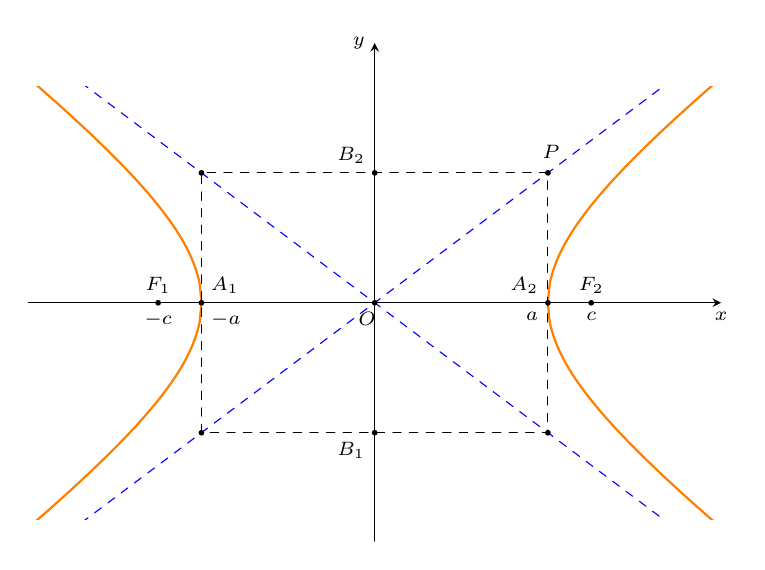
\begin{tikzpicture}[>=stealth,scale=.55, line join=round, line cap=round,font=\scriptsize]
		\draw[->] (-8,0)--(0.25,0)node[below left]{$ O $}--(8,0) node [below]{$x$};
		\draw[->] (0,-5.5)--(0,6) node [left]{$y$};
		%Hypebol
		\clip (-8,-5) rectangle (8,5);
		\draw[orange,thick,smooth,samples=100,domain=4:8] plot(\x,{3*sqrt(\x*\x/16-1)});
		\draw[orange,thick,smooth,samples=100,domain=-4:-8] plot(\x,{3*sqrt(\x*\x/16-1)});
		\draw[orange,thick,smooth,samples=100,domain=4:8] plot(\x,{-3*sqrt(\x*\x/16-1)});
		\draw[orange,thick,smooth,samples=100,domain=-4:-8] plot(\x,{-3*sqrt(\x*\x/16-1)});
		%Hình chữ nhật cơ sở
		\draw [dashed] (-4,-3)--(-4,3)--(4,3)--(4,-3)--(-4,-3);
		%Đường tiệm cận
		
		\draw[dashed,smooth,blue,samples=100,domain=-8:8] plot(\x,{-(3/4)*\x});
		\draw (-5,3.2)node[above right]{ };
		\draw[dashed,smooth,blue,samples=100,domain=-8:8] plot(\x,{(3/4)*\x});
		\draw (4.5,3.1)node[above left]{$ P $};
		%Đỉnh
		\draw [fill=black] (-4,0)node[above right]{$ A_1 $}circle(1.5pt) (4,0)node[above left]{$ A_2 $}circle(1.5pt) (-5,0)node[above]{$ F_1 $}circle(1.5pt) (5,0)node[above]{$ F_2 $}circle(1.5pt) (0,3)node[above left]{$ B_2 $}circle(1.5pt) (0,-3)node[below left]{$ B_1 $}circle(1.5pt) (-4,0)node[below right]{$ -a $} (4,0)node[below left]{$ a$} (-5,0)node[below]{$ -c $} (5,0)node[below]{$ c $} (0,0)circle(1.5pt) (-4,-3)circle(1.5pt) (-4,3)circle(1.5pt) (4,-3)circle(1.5pt) (4,3)circle(1.5pt);
	\end{tikzpicture}
\end{center}
\end{dang}
\begin{note}
	\begin{itemize}
		\item $(H)$ cắt $Ox$ tại hai điểm $A_1(-a; 0)$ và $A_2(a; 0)$. Nếu ta vẽ hai điểm $B_1(0; -b)$ và $B_2(0; b)$ vào hình chữ nhật $OA_2PB_2$ thì $OP=\sqrt{a^2+b^2}=c$.
		\item Các điểm $A_1, A_2$ gọi là các đỉnh của hypebol.
		\item Đoạn thẳng $A_1A_2 = 2a$ gọi là trục thực, đoạn thẳng $B_1B_2 = 2b$ gọi là trục ảo của hypebol.
		\item Giao điểm $O$ của hai trục là tâm đối xứng của hypebol.
		\item  Nếu $M(x; y) \in (H)$ thì $x \leq -a$  hoặc  $x \geq a$.
	\end{itemize} 
\end{note}

\subsubsection{Các ví dụ}
\begin{vd}%Ví dụ 1
	\begin{enumerate}
		\item Tìm tâm sai của hypebol $3x^2 - y^2 = 12$.
		\item 	 Cho hypebol $(H) \colon$ $\dfrac{x^2}{4}-\dfrac{y^2}{9}=1$. Tìm tọa độ đỉnh, tiêu điểm, tâm sai và hai tiệm cận của $(H)$. 
	\end{enumerate}
	
	\loigiai{
		\begin{enumerate}
			\item $3x^2 - y^2 = 12 \Leftrightarrow \dfrac{x^2}{4}-\dfrac{y^2}{12}=1$.\\
			Ta có  $\heva{&a^2=4\\&b^2=12} \Rightarrow c= \sqrt{a^2+b^2}=4$.\\
			Do đó, hypebol có tâm sai là $ e=\dfrac{c}{a}=\dfrac{4}{2}=2 $.
			\item 
			Ta có $ \heva{&a^2=4\\&b^2=9}\Rightarrow a=2, b=3, c=\sqrt{a^2+b^2}=\sqrt{13} $.\\
			Do đó có các tiêu điểm $F_1(-\sqrt{13}; 0)$ và $F_2(\sqrt{13};0)$.
			Các đỉnh của hypebol là $ A_1(-4,0) $, $ A_2(4,0) $.\\
			Các đường tiệm cận của hypebol là $ y=-\dfrac{3}{2}x $ và $ y=\dfrac{3}{2}x $.
		\end{enumerate}
	}
\end{vd}
\begin{vd}%Ví dụ 2
	Cho hypebol $(H)$ có một tiêu điểm $F_2(8; 0)$ và $(H)$ đi qua điểm $A(5; 0)$. Viết phương trình chính tắc của hypebol $(H)$.
	\loigiai{
		Phương trình chính tắc của hypebol có dạng $$ \dfrac{x^2}{a^2}-\dfrac{y^2}{b^2}=1. $$
		Vì hypebol đi qua điểm $ A(5; 0) $ nên ta có $$ \dfrac{25}{a^2}-\dfrac{0^2}{b^2}=1\Rightarrow a^2=25\Rightarrow a=5. $$
		Do $(H)$ có một tiêu điểm $F_2(8; 0)$ nên $c=8$.
		Do đó $ b^2=c^2-a^2=8^2-5^2=39 $.\\
		Vậy phương trình chính tắc của hypebol là $ \dfrac{x^2}{25}-\dfrac{y^2}{39}=1 $.
	}
\end{vd}

\subsubsection{Câu hỏi trắc nghiệm}
\begin{ex}
	Parabol có phương trình $y^2=\sqrt{2}x$ có
	\choice
	{tiêu điểm $F(\sqrt{2};0)$}
	{đường chuẩn $\Delta\colon x=-\dfrac{\sqrt{2}}{2}$}
	{tham số tiêu $p=\sqrt{2}$}
	{\True khoảng cách từ tiêu điểm đến đường chuẩn là $\mathrm{d}(F,\Delta)=\dfrac{\sqrt{2}}{2}$}
	\loigiai{
		Ta có $y^2=\sqrt{2}x=2px\Rightarrow p=\dfrac{\sqrt{2}}{2}$. \\
		Do đó, parabol có tiêu điểm $F\left(\dfrac{\sqrt{2}}{4};0\right)$ và đường chuẩn $\Delta\colon x=-\dfrac{\sqrt{2}}{4}$. \\
		Suy ra khoảng cách từ tiêu điểm đến đường chuẩn là $\mathrm{d}(F,\Delta)=\dfrac{\sqrt{2}}{2}$.
	}
\end{ex}
\begin{ex}
	Đường thẳng nào là đường chuẩn của parabol $y^2=\dfrac{3}{2}x$?
	\choice
	{$x=\dfrac{3}{2}$}
	{\True $x=-\dfrac{3}{8}$}
	{$x=-\dfrac{3}{4}$}
	{$x=\dfrac{3}{4}$}
	\loigiai{
		Ta có $y^2=\dfrac{3}{2}x=2px\Rightarrow p=\dfrac{3}{4}$.\\
		Đường chuẩn của parabol là $x=-\dfrac{3}{8}$.
	}
\end{ex}
\begin{ex}
	Khoảng cách từ tiêu điểm đến đường chuẩn của parabol $y^2=\sqrt{3}x$ bằng
	\choice
	{\True $\dfrac{\sqrt{3}}{2}$}
	{$\sqrt{3}$}
	{$\dfrac{\sqrt{3}}{4}$}
	{$\dfrac{\sqrt{3}}{8}$}
	\loigiai{
		Ta có $y^2=\sqrt{3}x=2px\Rightarrow p=\dfrac{\sqrt{3}}{2}$.\\
		Vậy khoảng cách từ tiêu điểm đến đường chuẩn của parabol bằng $\dfrac{\sqrt{3}}{2}$.
	}
\end{ex}
\begin{ex}
	Phương trình chính tắc của parabol mà khoảng cách từ đỉnh tới tiêu điểm bằng $\dfrac{3}{4}$ là
	\choice
	{$y^2=\dfrac{3}{4}x$}
	{$y^2=\dfrac{3}{2}x$}
	{\True $y^2=3x$}
	{$y^2=6x$}
	\loigiai{
		Theo giả thiết, ta có $\dfrac{p}{2}=\dfrac{3}{4}\Rightarrow p=\dfrac{3}{2}$.\\
		Do đó phương trình của parabol là $y^2=2px=3x$.
	}
\end{ex}

\begin{ex}%Câu 5%[0H7B6-5]
	Hypebol có nửa trục thực là $4$, tiêu cự bằng $10$ có phương trình chính tắc là
	\choice
	{\True $\dfrac{x^2}{16}-\dfrac{y^2}{9}=1$}
	{$\dfrac{y^2}{16}+\dfrac{x^2}{9}=1$}
	{$\dfrac{x^2}{16}-\dfrac{y^2}{25}=1$}
	{$\dfrac{y^2}{16}-\dfrac{x^2}{9}=1$}
	\loigiai{
		Ta có $\hoac{&a=4\\&2c=10\\&b^2=c^2-a^2} \Rightarrow \hoac{&a=4\\&c=5\\&b=3.}$\\
		Vậy phương trình chính tắc của Hypebol là $\dfrac{x^2}{16}-\dfrac{y^2}{9}=1$.
	}
\end{ex}

\begin{ex}%Câu 6%[0H7B6-5]
	Hypebol có tâm sai $\mathrm{e}=\sqrt{5}$ và đi qua điểm $(1;0)$ có phương trình chính tắc là
	\choice
	{$\dfrac{y^2}{1}+\dfrac{x^2}{4}=1$}
	{\True $\dfrac{x^2}{1}-\dfrac{y^2}{4}=1$}
	{$\dfrac{y^2}{1}-\dfrac{x^2}{4}=1$}
	{$\dfrac{x^2}{4}-\dfrac{y^2}{25}=1$}
	\loigiai{
		Xét Hypebol $(H)$ có phương trình chính tắc là $\dfrac{x^2}{a^2}-\dfrac{y^2}{b^2}=1 \qquad (H)$.\\
		Từ giả thuyết ta có  $\dfrac{c}{a}=\sqrt{5} \Rightarrow c^2=5a^2$.\\
		Mà $c^2=a^2+b^2 \Rightarrow 4a^2=b^2$.\\
		Mặt khác $H$ đia qua $(1;0)$ nên $\dfrac{1}{a^2}=1 \Rightarrow a^2=1 \Rightarrow b^2=4$.\\
		Vậy phương trình chính tắc của Hypebol là $\dfrac{x^2}{1}-\dfrac{y^2}{4}=1$.
	}
\end{ex}

\begin{ex}%Câu 7%[0H7B6-4]
	Phương trình hai tiệm cận $y= \pm \dfrac{2}{3}x$ là của phương trình chính tắc $(H)$ nào sau đây?
	\choice
	{$\dfrac{x^2}{4}-\dfrac{y^2}{9}=1$}
	{$\dfrac{x^2}{2}-\dfrac{y^2}{3}=1$}
	{\True $\dfrac{x^2}{9}-\dfrac{y^2}{4}=1$}
	{$\dfrac{x^2}{3}-\dfrac{y^2}{2}=1$}
	\loigiai{
		Hypebol có hai đường tiệm cận $y= \pm \dfrac{2}{3}x \Rightarrow \heva{&a=3\\&b=2.}$\\
		Vậy phương trình hai tiệm cận $y= \pm \dfrac{2}{3}x$ là của phương trình chính tắc $\dfrac{x^2}{9}-\dfrac{y^2}{4}=1$.
	}
\end{ex}

\begin{ex}%Câu 8%[0H7B6-3]
	Cho đường thẳng $ \Delta $ và một điểm $F$ không thuộc $ \Delta $. Tập hợp các điểm $M$ sao cho $MF=\dfrac{1}{\sqrt{2}}\mathrm{d}(M, \Delta)$ là một
	\choice
	{\True elip}
	{hypebol}
	{parabol}
	{đường tròn}
	\loigiai{
		Ta có $\dfrac{MF}{\mathrm{d}(M, \Delta)} = \dfrac{1}{\sqrt{2}}$. Nên quỹ tích các điểm $M$ là một elip.
	}
\end{ex}

\begin{ex}%Câu 9
	Viết phương trình chính tắc của Hypebol, biết giá trị tuyệt đối hiệu các bán kính qua tiêu của điểm $M$ bất kỳ trên hypebol là $8$, tiêu cự bằng $10$.
	\choice
	{\True $\dfrac{x^2}{16}-\dfrac{y^2}{9}=1$}
	{$\dfrac{x^2}{4}-\dfrac{y^2}{3}=1$}
	{$\dfrac{x^2}{4}+\dfrac{y^2}{3}=1$}
	{$\dfrac{x^2}{16}-\dfrac{y^2}{9}=1$ hoặc $-\dfrac{x^2}{9}+\dfrac{y^2}{16}=1$}
	\loigiai{
	Theo đề bài $\left|MF_1-MF_2\right|=2a=8\Rightarrow a=4$, tiêu cự $2c=10\Rightarrow c=5$, suy ra $b^2=c^2-a^2=5^2-4^2=9$.\\
	Phương trình chính tắc của Hypebol là $\dfrac{x^2}{16}-\dfrac{y^2}{9}=1$.
	}
\end{ex}

\begin{ex}%Câu 10
	Viết phương trình của Hypebol có $2c = 10, 2a = 8$ và tiêu điểm nằm trên trục $Ox$.
	\choice
	{\True $\dfrac{x^2}{16}-\dfrac{y^2}{9}=1$}
	{$\dfrac{x^2}{4}-\dfrac{y^2}{3}=1$}
	{$\dfrac{x^2}{4}+\dfrac{y^2}{3}=1$}
	{$\dfrac{x^2}{16}-\dfrac{y^2}{9}=1$ hoặc $-\dfrac{x^2}{9}+\dfrac{y^2}{16}=1$}
	\loigiai{
	Từ $2c=10\Rightarrow c=5$, $2a=8\Rightarrow a=4$, suy ra $b=\sqrt{c^2-a^2}=9$.\\
	Suy ra phương trình Hypebol là $\dfrac{x^2}{16}-\dfrac{y^2}{9}=1$.
	}
\end{ex}

\begin{ex}%Câu 11
	Hypebol $\dfrac{x^2}{16}-\dfrac{y^2}{9}=1$ có hai tiêu điểm là
	\choice
	{$F_1(-2;0);F_2(2;0)$}
	{$F_1(-3;0);F_2(3;0)$}
	{$F_1(-4;0);F_2(4;0)$}
	{\True $F_1(-5;0);F_2(5;0)$}
	\loigiai{
	Từ phương trình $(H)\colon \dfrac{x^2}{16}-\dfrac{y^2}{9}=1$ suy ra $a=4$, $b=3$, $c=\sqrt{a^2+b^2}=5$.\\
	Do đó hai tiêu điểm của Hypebol là $F_1(-5;0);F_2(5;0)$.
	}
\end{ex}

\subsection{Parabol}
\begin{dang}{Parabol}
\immini{
	\begin{dn}[Parabol]
		Cho một điểm $F$ và một đường thẳng $\Delta$ cố định không đi qua $F$. Parabol $(P)$ là tập hợp các điểm $M$ cách đều $F$ và $\Delta$.\\
		$F$ gọi là \textbf{tiêu điểm} và $\Delta$ gọi là \textbf{đường chuẩn} của parabol $(P)$.
	\end{dn}
}{
	\begin{tikzpicture}[scale=1, font=\footnotesize, line join=round, line cap=round, >=stealth]
		\def\xm{-1.3};
		\pgfmathsetmacro\ym{0.5*(\xm)^2};
		\path
		(0,0) coordinate (O)
		(0,0.5) coordinate (F)
		(\xm,\ym) coordinate (M)
		;
		%		\draw[->] (-2,0)--(2,0) node[above]{$x$};
		%		\draw[->] (0,-1.5)--(0,2.5) node[left]{$y$};
		\draw[smooth, samples=200, domain=-2:2] plot (\x,{0.5*(\x)^2});
		\draw (-2,-0.5)--(2,-0.5) node[below]{$\Delta$};
		%		\draw[fill=black] (O) circle(1pt)++(-0.2,-0.2) node{$O$};
		\draw[fill=black] (F) circle(1pt) node[right]{$F$};
		\draw[fill=black] (M) circle(1pt)++(0.2,0.3) node{$M$};
		\draw (F)--(M)--(\xm,-0.5);
		\draw ($(\xm,-0.5)+(0.2,0)$)|-($(\xm,-0.5)+(0,0.2)$);
	\end{tikzpicture}
}
\immini{
	\begin{dl}[Phương trình chính tắc]
		Cho parabol $(P)$ có tiêu điểm $F$ và đường chuẩn $\Delta$. Gọi khoảng cách từ tiêu điểm đến đường chuẩn là $p$, hiển nhiên $p > 0$.\\
		Chọn hệ trục tọa độ $Oxy$ sao cho $F\left( \dfrac{p}{2};0 \right)$ và $\Delta: x+\dfrac{p}{2}=0.$
		$$M(x; y)\in(P) \Leftrightarrow y^2 = 2px\quad (3).$$
		Phương trình $(3)$ gọi là phương trình chính tắc của parabol.
		
	\end{dl}
}{
	\begin{tikzpicture}[scale=1, font=\footnotesize, line join=round, line cap=round, >=stealth]
		\def\xm{-1.3};
		\pgfmathsetmacro\ym{0.5*(\xm)^2};
		\path
		(0,0) coordinate (O)
		(0.5,0) coordinate (F)
		(\xm,\ym) coordinate (N)
		(\ym,-\xm) coordinate (M)
		;
		\draw[->] (-1.5,0)--(2.5,0) node[above]{$x$};
		\draw[->] (0,-2)--(0,2) node[right]{$y$};
		\draw[rotate=-90,smooth, samples=200, domain=-2:2] plot (\x,{0.5*(\x)^2});
		\draw (-0.5,2)--(-0.5,-2) node[left]{$\Delta$};
		\draw[fill=black] (O) circle(1pt)++(-0.2,-0.2) node{$O$};
		\draw[fill=black] (F) circle(1pt) +(0.5,-0.4) node{$F\left(\dfrac{p}{2};0\right)$};
		\draw[fill=black] (M) circle(1pt) node[right]{$M$};
		\draw (F)--(M)--(-0.5,-\xm);
		\draw ($(-0.5,-\xm)+(0.2,0)$)|-($(-0.5,-\xm)+(0,-0.2)$);
	\end{tikzpicture}
}
\end{dang}
\begin{note}
	\textbf{Chú ý:}
	\begin{itemize}
		\item $O$ gọi là \textbf{đỉnh} của parabol $(P)$.
		\item $Ox$ gọi là \textbf{trục đối xứng} của parabol $(P)$.
		\item $p$ gọi là \textbf{tham số tiêu} của parabol $(P)$.
		\item Nếu $M(x;y)\in (P)$ thì $x\ge 0$ và $M'(x;-y)\in (P)$.
	\end{itemize}
\end{note}
\subsubsection{Các ví dụ}
\begin{vd}
	\begin{listEX}
		\item Tìm tiêu điểm, phương trình đường chuẩn của parabol $y^2 =\dfrac{1}{2} x$.
		\item Tìm tiêu điểm, phương trình đường chuẩn của parabol $y^2 = 4x$.
	\end{listEX}
	\loigiai{
		\begin{listEX}
			\item Do $p=\dfrac{1}{4}$ nên tiêu điểm là $F\left(\dfrac{1}{8};0 \right)$ và đường chuẩn là $\Delta: x+\dfrac{1}{8}=0$. 
			\item Do $p=2$ nên tiêu điểm là $F\left(1;0 \right)$ và đường chuẩn là $\Delta: x+1=0$. 
	\end{listEX}
}
\end{vd}
\begin{vd}
	Viết phương trình chính tắc của parabol $(P)$, biết $(P)$ có đường chuẩn $\Delta: x+4=0$.
	\loigiai{
		Do $\dfrac{p}{2}=4$ nên $p=8$. Do đó $(P)\colon y^2=16x$. 
	}
\end{vd}
\subsubsection{Câu hỏi trắc nghiệm}
\setcounter{ex}{0}
\begin{ex}%Câu 1
	Parabol có phương trình  $y^2 = \sqrt{2}x$ có
	\choice
	{$F(\sqrt{2};0)$}
	{\True $\Delta \colon x=-\dfrac{\sqrt{2}}{4}$}
	{$p=\sqrt{2}$}
	{$\mathrm{d}(F, \Delta)=\dfrac{\sqrt{2}}{2}$}
	\loigiai{
		Phương trình parabol $y^2 = \sqrt{2}x$  có $p=\dfrac{\sqrt{2}}{2}$.\\
		Do đó phương trình đường chuẩn là $\Delta \colon x=-\dfrac{\sqrt{2}}{4}$.
	}
\end{ex}

\begin{ex}%Câu 2
	Đường thẳng nào là đường chuẩn của parabol $y^2 = \dfrac{3}{2}x$?
	\choice
	{$x = \dfrac{3}{2}$}
	{$x = -\dfrac{3}{4}$}
	{\True $x = -\dfrac{3}{8}$}
	{$x = \dfrac{3}{4}$}
	\loigiai{
		Phương trình parabol $y^2 = \dfrac{3}{2}x$  có $p=\dfrac{3}{4}$.\\
		Do đó phương trình đường chuẩn là $\Delta \colon x=-\dfrac{3}{8}$.
	}
\end{ex}

\begin{ex}%Câu 3
	Khoảng cách từ tiêu điểm đến đường chuẩn của parabol $y^2=\sqrt{3}x$ là
	\choice
	{\True $\mathrm{d}(F, \Delta)=\dfrac{\sqrt{3}}{2}$}
	{$\mathrm{d}(F, \Delta)=\sqrt{3}$}
	{$\mathrm{d}(F, \Delta)=\dfrac{\sqrt{3}}{4}$}
	{$\mathrm{d}(F, \Delta)=\dfrac{\sqrt{3}}{8}$}
	\loigiai{
		Khoảng cách từ tiêu điểm đến đường chuẩn của parabol $y^2=\sqrt{3}x$ là $p=\dfrac{\sqrt{3}}{2}$.
	}
\end{ex}

\begin{ex}%Câu 4
	Phương trình chính tắc của parabol mà khoảng cách từ đỉnh tới tiêu điểm bằng $\dfrac{3}{4}$ là
	\choice
	{$y^2=\dfrac{3}{4}x$}
	{\True $y^2=\dfrac{3}{2}x$}
	{$y^2=3x$}
	{$y^2=6x$}
	\loigiai{
		Ta có $\dfrac{p}{2}=\dfrac{3}{4}\Rightarrow p=\dfrac{3}{2}$.\\
		Vậy phương trình chính tắc của parabol là $y^2=\dfrac{3}{2}x$.
	}
\end{ex}


\begin{ex}%Câu 5
	Cho parabol $(P)\colon y^2=4x$ có tiêu điểm là $F$. Gọi $M$ là điểm thuộc $(P)$ thỏa mãn $MF = 3$. Hoành độ của $M$ bằng
	\choice
	{$1$}
	{$3$}
	{$\dfrac{3}{2}$}
	{\True $2$}
	\loigiai{
		\immini{Ta có $y^2=4x\Rightarrow p=2 \Rightarrow \Delta\colon x + 1 = 0$ là phương trình đường chuẩn của $(P)$.\\
			Vì $M\in (P)$ nên $x_M >0$ và $$\mathrm{d}(M;\Delta)=MF\Leftrightarrow \mathrm{d}(M;\Delta) = 3
			\Leftrightarrow \mathrm{d}(M;Oy)=2\Rightarrow x_M =2.$$
		}{
			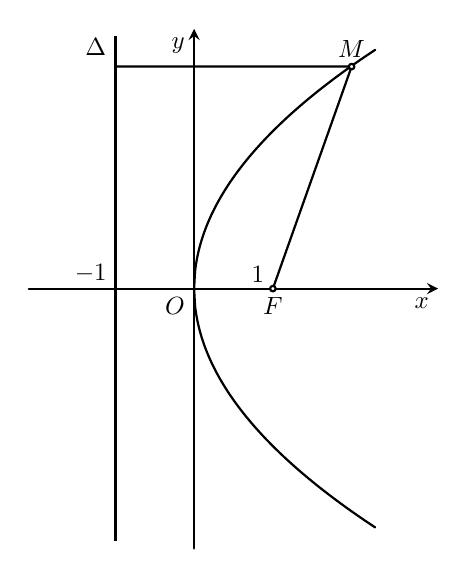
\begin{tikzpicture}[line join=round, line cap=round,>=stealth,thick]
				\tikzset{every node/.style={scale=0.9}}
				\draw[->] (-2.1,0)--(3.1,0) node[below left] {$x$};
				\draw[->] (0,-3.3)--(0,3.3) node[below left] {$y$};
				\draw (0,0) node [below left] {$O$};
				\draw (1,0) node [below] {$F$};
				\draw[fill=black] (2,2.82) node [above] {$M$};
				\draw (-1,2.82)--(2,2.82)--(1,0);
				\foreach \x in {-1,1}
				\draw[thin] (\x,1pt)--(\x,-1pt) node [above left] {$\x$};
				\begin{scope}
					\clip (-2,-3.2) rectangle (3,3.2);
					\draw[samples=200,domain=0:2.3,smooth,variable=\x] plot (\x,{2*sqrt((\x))});
					\draw[samples=200,domain=0:2.3,smooth,variable=\x] plot (\x,{-2*sqrt((\x))});
					\draw[-] (-1,-3.3)--(-1,3.3) node[below left] {$\Delta$};
				\end{scope}
				\draw[fill=white]  (2,2.82)   (1,0)  circle (1pt);
				\draw[fill=white]  (2,2.82)  circle (1pt);
			\end{tikzpicture}
		}
	}
\end{ex}

\begin{ex}%Câu 6
	Gọi $MN$ là một dây cung đi qua tiêu điểm $F$ của parabol $(P)$ thỏa mãn $MN$ vuông góc với $Ox$ và $MN =3$. Khoảng cách từ tiêu điểm đến đường chuẩn của $(P)$ bằng
	\choice
	{$12$}
	{$3$}
	{$6$}
	{\True đáp số khác}
	\loigiai{
		\immini{Ta có  $M, N \in (P); MN \perp Ox$ và $Ox$ là trục đối xứng của $(P)$ nên $x_M=x_N$ và $y_M=-y_N$.\\
			Không mất tính tổng quát, giả sử $y_M=b>0\Rightarrow y_N=-b$ .\\
			Vì $MN=3$ nên $2b=3 \Leftrightarrow b=\dfrac{3}{2}$. \\
			Do $MN$ đi qua $F$ và $MN\perp Ox$ nên $MF=y_M=\dfrac{3}{2}$\\
			$\Rightarrow \mathrm{d}(F;\Delta) = \mathrm{d}(M;\Delta)=MF=\dfrac{3}{2}$ (Với $\Delta$ là đường chuẩn của $(P)$).
		}{
			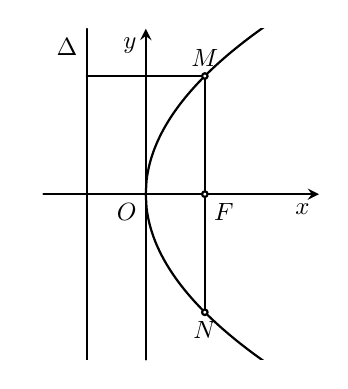
\begin{tikzpicture}[line join=round, line cap=round,>=stealth,thick]
				\tikzset{every node/.style={scale=0.9}}
				\draw[->] (-1.3,0)--(2.2,0) node[below left] {$x$};
				\draw[->] (0,-2.1)--(0,2.1) node[below left] {$y$};
				\draw (0,0) node [below left] {$O$};
				\draw (3/4,0) node [below right] {$F$};
				\draw[fill=black] (3/4,3/2) node [above] {$M$};
				\draw[fill=black] (3/4,-3/2) node [below] {$N$};
				\draw (-3/4,3/2)--(3/4,3/2)--(3/4,-3/2);
				\begin{scope}
					\clip (-1.5,-2.1) rectangle (2.2,2.1);
					\draw[samples=200,domain=0:2,smooth,variable=\x] plot (\x,{sqrt(3)*sqrt((\x))});
					\draw[samples=200,domain=0:2,smooth,variable=\x] plot (\x,{-sqrt(3)*sqrt((\x))});
					\draw[-] (-3/4,-2.1)--(-3/4,2.1) node[below left] {$\Delta$};
				\end{scope}
				\draw[fill=white]  (3/4,3/2) circle (1pt);
				\draw[fill=white]  (3/4,-3/2) circle (1pt);
				\draw[fill=white]  (3/4,0)  circle (1pt);
			\end{tikzpicture}
		}
	}
\end{ex}

\begin{ex}%Câu 7
	Cho parabol $(P)\colon y^2=16x$. Một đường thẳng đi qua tiêu điểm $F$ của $(P)$, có hệ số góc bằng $1$, cắt $(P)$ tại $M$ và $N$. Độ dài $MN$ bằng
	\choice
	{$28$}
	{\True $32$}
	{$40$}
	{$20$}
	\loigiai{
		Ta có $y^2=16x = 2\cdot 8 \cdot x \Rightarrow p=8$. Suy ra tiêu điểm của $(P)$ là $F\left(4;0\right)$.\\
		Gọi $d$ là đường thẳng đi qua $F(4;0)$ và có hệ số góc bằng $1$. Phương trình của $d$ là
		$$y=1(x-4)+0\Leftrightarrow y= x-4.$$
		Tọa độ giao điểm của $d$ và $(P)$ là nghiệm của hệ phương trình 
		$$\heva{&y^2=16x\\&y=x-4} \Leftrightarrow \heva{&y^2-16y -64=0\\&x=y+4}\Leftrightarrow \heva{&\hoac{&y=8-8\sqrt{2}\\& y=8+8\sqrt{2}}\\&x=y+4.}$$
		Suy ra tọa độ hai giao điểm là $M\left(12-8\sqrt{2};8-8\sqrt{2}\right)$ và $N\left(12+8\sqrt{2};8+8\sqrt{2}\right)$.\\
		Vậy $MN=32$.
	}
\end{ex}

\begin{ex}%Câu 8
	Đường thẳng nào là đương chuẩn của parabol $y^2=4x$?
	\choice
	{$x=-2$}
	{\True $x=-1$}
	{$x=4$}
	{$x=\pm 1$}
	\loigiai{
		Ta có $y^2=4x = 2\cdot 2 \cdot x \Rightarrow p=2$. Suy ra phương trình đường chuẩn là $x=-\dfrac{p}{2}=-1$.
	}
\end{ex}

\begin{ex}%Câu 9
	Viết phương trình Parabol $(P)$ có tiêu điểm $F(3;0)$ và đỉnh là gốc tọa độ $O$.
	\choice
	{$y^2=-2x$}
	{$y^2=6x$}
	{\True $y^2=12x$}
	{$y=x^2+\dfrac{1}{2}$}
	\loigiai{
	Phương trình $(P)$ có dạng $y^2=2px$.\\
	Từ tiêu điểm $F(3;0)$ suy ra $\dfrac{p}{2}=3\Rightarrow p=6$.\\
	Vậy phương trình cần tìm là $y^2=12x$.
	}
\end{ex}

\begin{ex}%Câu 10
	Cho điểm $A(3;0)$, gọi $M$ là một điểm tuỳ ý trên $(P): y^2 = x$. Tìm giá trị nhỏ nhất của $AM$.
	\choice
	{$4$}
	{$\dfrac{5}{2}$}
	{$\dfrac{9}{2}$}
	{\True $\dfrac{\sqrt{11}}{2}$}
	\loigiai{
	Điểm $M$ thuộc $(P)$ nên tọa độ $M$ có dạng $M(b^2;b)$.\\
	Độ dài $AM=\sqrt{(b^2-3)^2+b^2}=\sqrt{b^4-5b^2+9}=\sqrt{\left(b^2-\dfrac{5}{2}\right)^2+\dfrac{11}{4}}\ge \dfrac{\sqrt{11}}{2}$.\\
	Do đó $AM$ nhỏ nhất bằng $\dfrac{\sqrt{11}}{2}$ khi $M\left(\dfrac{\sqrt{10}}{2};\dfrac{5}{2}\right)$.
	}
\end{ex}

\begin{ex}%Câu 11
	Cho $M$ là một điểm thuộc $(P)\colon y^2 = 64x$, $N$ là một điểm thuộc đường thẳng $(d)\colon 4x + 3y + 46 = 0$. Tìm giá trị nhỏ nhất của đoạn thẳng $MN$.
	\choice
	{\True $2$}
	{$4$}
	{$\dfrac{5}{2}$}
	{$\dfrac{3}{2}$}
	\loigiai{
	Điểm $M\left(\dfrac{y^2}{64};y\right)$ thuộc parabol.\\
	Khoảng cách từ $M$ đến $d$ là $$\mathrm{\,d}(M,d)=\dfrac{\left|4\cdot \dfrac{y^2}{64}+3y+46\right|}{\sqrt{4^2+3^2}}=\dfrac{1}{80}\cdot  \left|y^2+48y+736\right|=\dfrac{1}{80}\cdot \left|(y-24)^2+160\right|\le \dfrac{160}{80}=2.$$
	Giá trị nhỏ nhất đạt được khi $M(9;24)$, $N\left(-\dfrac{391}{25};{\dfrac{138}{25}}\right)$.
	}
\end{ex}
\Closesolutionfile{ans}

\subsection{Bài toán thực tế}

\begin{bt}%[BG2-2022-Huỳnh Xuân Tín]
	Mặt Trăng chuyển động theo một quỹ đạo là hình elip nhận tâm Trái Đất là một tiêu điểm. Các khoảng cách lớn nhất và nhỏ nhất từ các vị trí của Mặt Trăng đến tâm Trái Đất tương ứng là $400000$ km và $363000$ km (theo nssdc.gsfc.nasa.gov). Tìm tâm sai của quỹ đạo elip.
	\loigiai{
\immini{Gọi phương trình quỹ đạo elip có dạng $\dfrac{x^2}{a^2}+\dfrac{y^2}{b^2}=1$.\\
	Theo tính chất elip và theo giả thiết thì $A_1F_=363000$ và $A_2F_1=400000$.\\
Khi đó $\heva{&a-c=363000\\&a+c=400000}\Rightarrow\heva{&a=381500\\&c=18500.}$\\
Ta có $b=\sqrt{a^2-b^2}=381051{,}177$.\\
Vậy tâm sai của quỹ đạo là $e=\dfrac{c}{a}=0{,}0485499$.}{\begin{tikzpicture}[scale=1.2, font=\footnotesize, line join=round, line cap=round,>=stealth]
		\def \xmin{-2.7};
		\def \xmax{2.7};
		\def \ymin{-1.9};
		\def \ymax{2.0};
		\def \a{2.3};
		\def \b{1.5};
		\pgfmathsetmacro{\c}{sqrt((\a)^2-(\b)^2)};
		\draw[->] (\xmin, 0.) -- (\xmax+0.5,0.) node[anchor=north] {$x$};
		\draw[->] (0.,\ymin) -- (0.,\ymax) node[anchor=west] {$y$};
		%\clip(\xmin,\ymin) rectangle (\xmax,\ymax);
		\draw (0,0) ellipse ({\a} and {\b});
		\coordinate[label=above: Mặt Trăng] (M) at ($(0,0) + (60: {\a}  and {\b})$);
		\draw ({-\c},0) node[above, xshift=10pt] {$F_1$}circle(1pt) --(M)circle(1pt)--({\c},0)node[below, xshift=-5pt] {$F_2$}circle(1pt);
		\draw[fill=black] (0,0) circle (1pt) node[below left] {$O$};
			\draw[fill=black] ({-\a},0) circle (1pt) node[below left] {$A_1$};
			\draw[fill=black] ({\a},0) circle (1pt) node[below right] {$A_2$};
				\draw[fill=black] ({-\c},0) circle (1pt) node[below] {Trái Đất};
	\end{tikzpicture}
}}
\end{bt}


\begin{bt}%[BG2-2022-Huỳnh Xuân Tín]
	Với tâm sai khoảng $0{,}244$ quỹ đạo của sao Diêm Vương "dẹt" so với quỹ đạo của tám hình tinh trong hệ Mặt Trời. Nửa độ dài trục lớn của elip quỹ đạo là khoảng $590635\cdot 10^6$ km. Tìm khoảng cách gần nhất và khoảng cách xa nhất giữa sao Diêm Vương và tâm Mặt Trời ( tiêu điểm cuat quỹ đạo) (theo nssdc.gsfc.nasa.gov). 
	\loigiai{
Theo giả thiết ta có
 $$\heva{&e=0{,}244\\&a=590635\cdot 10^6}\Rightarrow c=e\cdot a=0{,}244\cdot 590635\cdot 10^6=144114{,}94\cdot 10^6.$$		
 Vậy khoảng cách gần nhất giữa sao Diêm Vương và tâm Mặt Trời $a-c=590635\cdot 10^6-144114{,}94\cdot 10^6=446520{,}06\cdot 10^6$ km.\\
 Khoảng cách xa nhất giữa sao Diêm Vương và tâm Mặt Trời $a+-c=590635\cdot 10^6+144114{,}94\cdot 10^6=734749{,}94\cdot 10^6$ km.
	}
\end{bt}


\begin{bt}%[BG2-2022-Huỳnh Xuân Tín]
\immini{Một phòng thì thầm có trần vòm elip với hai tiêu điểm ở độ cao $1{,6}$ m (so với mặt  sàn) và cách nhau $16$ m. Đỉnh của mái vòm cao $7{,}6$ m (hình bên). Hỏi âm thanh thì thầm từ một tiêu điểm thì sau bao nhiêu giây đến được tiêu điểm kia? Biết vận tốc âm thanh là $343{,}2$ m/s và làm tròn đáp số tới $4$ chữ số sau dấu phẩy.}{\begin{tikzpicture}[scale=1.2, font=\footnotesize, line join=round, line cap=round,>=stealth]
		\def \xmin{-2.7};
		\def \xmax{2.7};
		\def \ymin{-1.9};
		\def \ymax{2.0};
		\def \a{2.3};
		\def \b{1.5};
		\pgfmathsetmacro{\c}{sqrt((\a)^2-(\b)^2)};
		%	\draw[->] (\xmin, 0.) -- (\xmax+0.5,0.) node[anchor=north] {$x$};
		%	\draw[->] (0.,\ymin) -- (0.,\ymax) node[anchor=west] {$y$};
		%\clip(\xmin,\ymin) rectangle (\xmax,\ymax);
		%\draw (0,0) ellipse ({\a} and {\b});
		\coordinate[] (M) at ($(0,0) + (60: {\a}  and {\b})$);
		\draw[->] ({-\c},0)circle(1pt) --(M)circle(1pt)--({\c},0)circle(1pt);
	%	\draw[fill=black] (0,0) circle (1pt) node[below left] {$O$};
		%\draw[fill=black] ({-\a},0) circle (1pt) node[above left] {$A_1$};
	%	\draw[fill=black] ({\a},0) circle (1pt) node[above right] {$A_2$};
		\draw ({\a},0) arc (0:180:2.3cm and 1.5cm);
		\draw (-3.3,0)--(2.7,0);
		\draw (-3.3,-1)--(2.7,-1);
		\draw[<->][dashed] (-2.7,0)--(-2.7,-1); 
		\draw[fill=black] (-2.7,-0.5) node[left] {$1{,}6$m};	
		\draw[<->][dashed] (0,-1)--(0,1.5); 
		\draw[fill=black] (0,-0.5) node[right] {$7{,}6$m};			
\end{tikzpicture}}
	\loigiai{
\immini{Gọi phương trình quỹ đạo elip có dạng $\dfrac{x^2}{a^2}+\dfrac{y^2}{b^2}=1$.\\
	Ta có $2c=16\Rightarrow c=8$ và $b=7{,}6-1{,}6=6\Rightarrow a=\sqrt{b^2+c^2}=10$.\\
	Gọi một điểm $M$ bất kì trên mái vòm. Khi đó đường đi của âm thanh là $MF_1+MF_2=2a=20$.\\
	Vậy thời gian âm  thanh thì thầm từ một tiêu điểm đến được tiêu điểm kia là $20:343{,}2=0,0583$.
}{\begin{tikzpicture}[scale=1.2, font=\footnotesize, line join=round, line cap=round,>=stealth]
		\def \xmin{-2.7};
		\def \xmax{2.7};
		\def \ymin{-1.9};
		\def \ymax{2.0};
		\def \a{2.3};
		\def \b{1.5};
		\pgfmathsetmacro{\c}{sqrt((\a)^2-(\b)^2)};
	%	\draw[->] (\xmin, 0.) -- (\xmax+0.5,0.) node[anchor=north] {$x$};
	%	\draw[->] (0.,\ymin) -- (0.,\ymax) node[anchor=west] {$y$};
		%\clip(\xmin,\ymin) rectangle (\xmax,\ymax);
		%\draw (0,0) ellipse ({\a} and {\b});
		\coordinate[label=above: $M$] (M) at ($(0,0) + (60: {\a}  and {\b})$);
		\draw[->] ({-\c},0) node[below, xshift=10pt] {$F_1$}circle(1pt) --(M)circle(1pt)--({\c},0)node[below, xshift=-5pt] {$F_2$}circle(1pt);
		\draw[fill=black] (0,0) circle (1pt) node[below left] {$O$};
		\draw[fill=black] ({-\a},0) circle (1pt) node[above left] {$A_1$};
		\draw[fill=black] ({\a},0) circle (1pt) node[above right] {$A_2$};
		\draw ({\a},0) arc (0:180:2.3cm and 1.5cm);
\draw (-3.3,0)--(2.7,0);
\draw (-3.3,-1)--(2.7,-1);
\draw[<->][dashed] (-2.7,0)--(-2.7,-1); 
\draw[fill=black] (-2.7,-0.5) node[left] {$1{,}6$m};	
\draw[<->][dashed] (0,-1)--(0,1.5); 
\draw[fill=black] (0,-0.5) node[right] {$7{,}6$m};			
	\end{tikzpicture}
}		
	}
\end{bt}


\begin{bt}%[BG2-2022-Huỳnh Xuân Tín]
\immini{Một sao chổi đi qua hệ Mặt Trời theo quỹ đạo là một nhánh hypebol nhận tâm Mặt Trời là một tiêu điểm, khoảng cách gần nhất từ sao chổi này đến tâm Mặt Trời là $3\cdot 10^8$ km và tâm sai của quỹ đạo hypebol là $3{,}6$ (hình bên). Hãy lập phương trình chính tắc của hypebol chứa quỹ đạo, với một đơn vị đo trên mặt phẳng tọa độ tương ứng với $10^8$ km trên thực tế.}{\begin{tikzpicture}[scale=0.7, font=\footnotesize, line join=round, line cap=round, >=stealth,
		declare function={f(\a)=sqrt((1+(\a)^2/0.4671)*0.5329);},
		declare function={g(\b)=sqrt((1+(\b)^2/6.8684)*2.1316);}
		]
		%\draw[->] (-1,0)--(6,0) node [below]{$x$};
		%\draw[->] (0,-3)--(0,3) node [left]{$y$};
		\node at (0,0) [below left]{$O$};
		\fill (1.65197,1.38742) circle (1.5pt) node[above right]{Sao chổi};
		\draw[dashed] (3,0)node[above right]{$F_1$}--(1.65197,1.38742)--(0,0);
		\draw[fill=black] (3,0)circle (1pt) node[below] {Mặt Trời};
		\clip (-3.9,-2.9) rectangle (3.9,2.9);
		%	\draw[smooth] plot[domain=-3:3,variable=\a] ({-f(\a)},{\a});
		%	\draw[smooth] plot[domain=-3:3,variable=\a] ({f(\a)},{\a});
		%\draw[smooth] plot[domain=-3:3,variable=\b] ({-g(\b)},{\b});
		\draw[smooth] plot[domain=-3:3,variable=\b] ({g(\b)},{\b});
		%	\node at (3,2.3) [below]{$(H_1)$};
		%\node at (1.5,2.9) [below]{$(H_2)$};
		
\end{tikzpicture}}		
	\loigiai{
\immini{Chọn hệ trục tọa độ như hình vẽ (với một đơn vị đo trên mặt phẳng tọa độ tương ứng với $10^8$ km trên thực tế). Khi đó quỹ đạo có phương trình dạng $\dfrac{x^2}{a^2}-\dfrac{y^2}{b^2}=1$.\\
Ta có $\heva{&c-a=3\\&e=3{,}6}\Rightarrow\heva{&c-a=3\\&\dfrac{c}{a}=3{,}6}\Rightarrow\heva{&c=18\\&a=5.}$\\
Khi đó $b=\sqrt{c^2-a^2}=\sqrt{18^2-5^2}=\sqrt{299}$.\\
Vậy phương trình quỹ đạo hypebol cần tìm là $\dfrac{x^2}{25}-\dfrac{y^2}{299}=1$.}{\begin{tikzpicture}[scale=0.7, font=\footnotesize, line join=round, line cap=round, >=stealth,
		declare function={f(\a)=sqrt((1+(\a)^2/0.4671)*0.5329);},
		declare function={g(\b)=sqrt((1+(\b)^2/6.8684)*2.1316);}
		]
		\draw[->] (-1,0)--(6,0) node [below]{$x$};
		\draw[->] (0,-3)--(0,3) node [left]{$y$};
		\node at (0,0) [below left]{$O$};
		\fill (1.65197,1.38742) circle (1.5pt) node[above right]{Sao chổi};
		\draw[dashed] (3,0)node[above right]{$F_1$}--(1.65197,1.38742)--(0,0);
			\draw[fill=black] (3,0)circle (1pt) node[below] {Mặt Trời};
		\clip (-3.9,-2.9) rectangle (3.9,2.9);
	%	\draw[smooth] plot[domain=-3:3,variable=\a] ({-f(\a)},{\a});
	%	\draw[smooth] plot[domain=-3:3,variable=\a] ({f(\a)},{\a});
		%\draw[smooth] plot[domain=-3:3,variable=\b] ({-g(\b)},{\b});
		\draw[smooth] plot[domain=-3:3,variable=\b] ({g(\b)},{\b});
	%	\node at (3,2.3) [below]{$(H_1)$};
	%\node at (1.5,2.9) [below]{$(H_2)$};

\end{tikzpicture}}		
	}
\end{bt}

\begin{bt}%[BG2-2022-Huỳnh Xuân Tín]
\immini{Bốn trạm phát tín hiệu vô tuyến có vị trí $A$, $B$, $C$, $D$ theo thứ tự đó thẳng hàng và cách đều với khoảng cách $200$ km (hình bên). Tại một thời điểm, bốn trạm cùng phát tín hiệu với vận tốc $292000$ km/s. Một tàu thủy nhận được tín hiệu từ trạm $C$ trước $0{,}0005$ s so với tín hiệu từ trạm $B$ và nhận được tín hiệu từ trạm $D$ sớm $0{,} 0001$ s so với tín hiệu từ trạm $A$.}{\begin{tikzpicture}[scale=1.2, font=\footnotesize, line join=round, line cap=round, >=stealth]
		\draw[->] (-4,0)--(4,0) node [below]{$x$};
		\draw[->] (0,-1)--(0,3) node [left]{$y$};
		\node at (0,0) [below left]{$O$};
		\fill (-3,0) circle (1.5pt) node[below]{$A$};
		\fill (-1,0) circle (1.5pt) node[below]{$B$};
		\fill (1,0) circle (1.5pt) node[below]{$C$};
		\fill (3,0) circle (1.5pt) node[below]{$D$};
		\fill (2,2) circle (1.5pt) node[above]{$M$};
		\draw[dashed] (-3,0)--(2,2)--(-1,0) (3,0)--(2,2)--(1,0);
\end{tikzpicture}}
\begin{enumerate}
	\item Tính hiệu các khoảng cách từ tàu đến các trạm $B$, $C$.
	\item Tính hiệu các khoảng cách từ tàu đến các trạm $A$, $D$.
	\item Chọn hệ trục tọa độ $Oxy$ như hình bên(1 đơn vị trên mặt phẳng tọa độ ứng với $100$ km trên thực tế). Hãy lập phương trình chính tắc của hai hypebol đi qua vị trí $M$ của tàu. 
\end{enumerate} 
	\loigiai{
\begin{center}
		\begin{tikzpicture}[scale=1.2, font=\footnotesize, line join=round, line cap=round, >=stealth]
		\draw[->] (-4,0)--(4,0) node [below]{$x$};
		\draw[->] (0,-1)--(0,3) node [left]{$y$};
		\node at (0,0) [below left]{$O$};
		\fill (-3,0) circle (1.5pt) node[below]{$A$};
		\fill (-1,0) circle (1.5pt) node[below]{$B$};
		\fill (1,0) circle (1.5pt) node[below]{$C$};
		\fill (3,0) circle (1.5pt) node[below]{$D$};
		\fill (2,2) circle (1.5pt) node[above]{$M$};
		\draw[dashed] (-3,0)--(2,2)--(-1,0) (3,0)--(2,2)--(1,0);
	\end{tikzpicture}
\end{center}
\begin{enumerate}
	\item Chọn hệ trục như hình trên, và giả sử con tàu đang ở nhánh bên phải trục $Oy$.	Khi đó hai điểm $B$ và $C$ là hai tiêu điểm của một quỹ đạo hypebol. Do đó $MB-MC=2a=2OC=200$ km.
	\item Chọn hệ trục như hình trên, và giả sử con tàu đang ở nhánh bên phải trục $Oy$.	Khi đó hai điểm $A$ và $D$ là hai tiêu điểm của một quỹ đạo hypebol. Do đó $MB-MC=2a=2OD=600$ km.
	\item Chọn hệ trục tọa độ $Oxy$ như hình bên(1 đơn vị trên mặt phẳng tọa độ ứng với $100$ km trên thực tế). 
	\begin{itemize}
		\item Xét hypebol có hai tiêu điểm là $B$, $C$ suy ra $c=1$. Ta có một tàu thủy nhận được tín hiệu từ trạm $C$ trước $0{,}0005$ s so với tín hiệu từ trạm $B$ suy ra
		\[\dfrac{MB}{2920}-\dfrac{MC}{2920}=0{,}0005\Rightarrow MB-MC= \dfrac{73}{50}=2a\Rightarrow a=\dfrac{73}{100}.\]
		Khi đó $b=\sqrt{c^2-a^2}=\dfrac{\sqrt{4671}}{100}$.\\
		Vậy hypebol nhận $B$, $C$ là, tiêu điểm $H_1\colon \dfrac{x^2}{\dfrac{5329}{10000}}-\dfrac{y^2}{\dfrac{4671}{10000}}=1$.
		\item Xét hypebol có hai tiêu điểm là $A$, $D$ suy ra $c=3$. Ta có  nhận được tín hiệu từ trạm $D$ sớm $0{,} 001$ s so với tín hiệu từ trạm $A$ suy ra
		\[\dfrac{MA}{2920}-\dfrac{MD}{2920}=0{,}0001\Rightarrow MB-MC= \dfrac{73}{250}=2a\Rightarrow a=\dfrac{73}{500}.\]
		Khi đó $b=\sqrt{c^2-a^2}=\dfrac{\sqrt{2244671}}{500}$.\\
		Vậy hypebol nhận $A$, $D$ là, tiêu điểm $H_2\colon \dfrac{x^2}{\dfrac{5329}{250000}}-\dfrac{y^2}{\dfrac{2244671}{250000}}=1$.\\
		Khi đó tọa độ điểm $M$ là giao điểm của hai hypebol $H_1$ và $H_2$.
	\end{itemize}
\end{enumerate} 
	
	}
\end{bt}


% \begin{bt}%[BG2-2022-Huỳnh Xuân Tín]
% \immini{Xét đèn có bát đáy parabol với kích thước được thể hiện như hình bên. Dây tóc bóng đèn được đặt ở vị trí tiêu điểm. Tính khoảng cách từ dây tóc tới đỉnh bát đáy.}{{\includegraphics[scale=0.8]{"Pic/22-01"}}}
% 	\loigiai{
% \immini{Chọn hệ trục như hình vẽ, parabol có dạng $y^2=2px$.\\
% Ta có $OF=\dfrac{p}{2}$, $AB=30$, $OH=20$.\\
% Khi đó tọa độ điểm $A$ là $A(20;15)$ thuộc parabol nên
% \[15^2=2p\cdot 20\Rightarrow p=\dfrac{45}{8}.\]
% Vậy tiêu điểm của parabol là $P\left(\dfrac{45}{16};0\right)$.\\
% Do đó khoảng cách từ dây tóc tới đỉnh bát đáy là $\dfrac{45}{16}$. }{\begin{tikzpicture}[>=stealth,x=1cm,y=1cm,scale=.6]
% 		\coordinate[label=below left:$\scriptsize O$](O) at (0,0);
% 		\draw[->] (-1,0) -- (6,0) node[below] { $x$};
% 		\draw[->] (0,-4) -- (0,5) node[left] {$y$};
% 		\draw[thick,samples=150,smooth,domain=0:4] plot(\x,{2*\x^.5});
% 		\draw[thick,samples=150,smooth,domain=0:4] plot(\x,{-2*\x^.5});
% 		\fill (3,0)node[above right]{$F$} circle(1.5pt);
% 		\fill (4,4)node[above right]{$A$} circle(1.5pt);
% 			\fill (4,0)node[above right]{$H$} circle(1.5pt);
% 		\fill (4,-4)node[above right]{$B$} circle(1.5pt);
% 		\draw[dashed](4,4)--(4,-4);
% 		\draw(5,-2)--(1,-2)--(3,0)--(1,2)--(5,2);
% 		\draw(5,-1)--(.25,-1)--(3,0)--(.25,1)--(5,1);
% 		\draw[->](.25,1)--(4,1);
% 		\draw[->](1,2)--(4,2);
% 		\draw[->](.25,-1)--(4,-1);
% 		\draw[->](1,-2)--(4,-2);
% 		\draw[->](3,0)--(.25,1);
% 		\draw[->](3,0)--(.25,-1);
% 		\draw[->](3,0)--(1,2);
% 		\draw[->](3,0)--(1,-2);		
% \end{tikzpicture}}		
% 	}
% \end{bt}
% \textbf{Bài tập tương tự}
% \begin{bt}%[BG2-2022-Huỳnh Xuân Tín]
% \immini{Ăng-ten vệ tinh parabol ở hình bên có đầu thu đặt tại tiêu điểm, đường kính ăng-ten là $240$ cm, khoảng cách từ vị trí đặt đầu thu đến miệng ăng-ten là $130$ cm. Tính khoảng cách từ vị trí đặt đàu thu tới đỉnh ăng-ten.}{{\includegraphics[scale=0.8]{"Pic/22-02"}}}

% \end{bt}

\begin{bt}%[BG2-2022-Huỳnh Xuân Tín]
	Quỹ đạo chuyển động của sao chổi Halley là một elip, nhận Mặt Trời là một tiêu điểm, có tâm sai bằng $0{,}967$.
	\begin{enumerate}
		\item Giải thích vì sao ta có thể coi bất kì hình elip nào với tâm sai bằng $0{,}967$ là hình ảnh thu nhỏ của sao chổi Halley.
		\item Biết khoảng cách gần nhất từ sao chổi Halley đến tâm Mặt Trời là khoảng $88\cdot 10^6$ km, tính khoảng cách xa nhất (theo nssdc.gsfc.nasa.gov)
	\end{enumerate}
	
\end{bt}

\begin{bt}%[BG2-2022-Huỳnh Xuân Tín]%
	Một tàu vũ trụ nằm trong một quỹ đạo tròn và ở độ cao $148$km so với bờ mặt Trái Đất. Sau khi đạt được vận tốc cần thiết để thoát khỏa lực hấp dẫn của Trái Đất, tàu vũ trụ sẽ đi theo quỹ đạo parabol với tâm Trái Đất là tiêu điểm; điểm khởi đầu của quỹ đạo này là đỉnh parabol quỹ đạo.
	\begin{enumerate}
		\item Viết phương trình chính tắc của parabol quỹ đạo ($1$ đơn vị đo trên mặt phẳng tọa độ ứng với $1$ km thực tế, lấy bán kính Trái Đất là $6371$ km).
		\item Giải thích vì sao, kể từ khi đi vào quỹ đạo parabol, càng ngày, tàu vũ trụ càng cách xa Trái Đất.
	\end{enumerate}

\end{bt}

\begin{bt}%[BG2-2022-Huỳnh Xuân Tín]
	Khúc cua của một con đường có dạng hình parabol, điểm đầu vào khúc cua là $A$, điểm cuối là $B$, khoảng cách $AB=400$ m. Đỉnh của parabol $(P)$ của khúc cua cách đường  thẳng $AB$ một khoảng $20$ m và cách đều $A$, $B$.
	\begin{enumerate}
		\item Lập phương trình chính tắc của $(P)$, với $1$ đơn vị đo trong mặt phẳng tọa độ tương ứng với $1$ m thự tế.
		\item Lập phương trình chính tắc của $(P)$, với $1$ đơn vị đo trong mặt phẳng tọa độ tương ứng với $1$ km thự tế.
	\end{enumerate}
	
\end{bt}

